\section{Refactoring}
\label{sec:refactor}
Nach einer Analyse stehen in der Regel Änderungen im Code an. \textit{Refactoring}, oder zu Deutsch \textit{Refaktorierung}, beschreibt die nachträgliche Veränderung von Quellcode in Software. Konkret wird unter Beibehaltung des Verhaltens eines Programms eine verbesserte Struktur erzielt. Es ist also abgegrenzt von der Entwicklung neuer Funktionalitäten. Dies sollte vor allem bei großen Projekten ständiger Bestandteil sein. Schlechter Code erzeugt sonst immer größere Probleme und senkt somit auf Dauer die Produktivität \cite[S. 28]{martin2009}. Stattdessen sollte sauberer Code angestrebt werden. Dies bezieht sich sowohl auf Softwarearchitektur, als auch generelle Lesbarkeit von Code. Clean Code wird zum einen durch die im vorherigen Kapitel (\autoref{sec:codeanalyse}) genannten Kriterien, oder auch die ISO-Normen, auf höherer Ebene analysiert. Eine Sicht auf niedrigerer Ebene bietet Grady Booch, Autor von \textit{Object-Oriented Analysis and Design with Application}:
\begin{center}
	\textit{Sauberer Code ist einfach und direkt. Sauberer Code liest sich wie wohlgeschriebene Prosa. Sauberer Code verdunkelt niemals die Absicht des Designers, sondern ist voller griffiger (engl. crisp) Abstraktionen und geradliniger Kontrollstrukturen.} \cite[S. 34]{martin2009}
\end{center}
Durchgehend sauberer Code ist zum Beispiel aufgrund von sich verändernden Anforderungen schwer zu erreichen. Daher ist Refactoring ein derart wichtiger Prozess. Da Refactoring aber auch bedeutet, dass in dieser Zeit keine neuen Funktionen entwickelt werden, ist die Balance sehr wichtig.

\subsection{Betroffene Stellen}
\label{subsec:whereRefact}
Betroffen sind zum Einen die Ergebnisse von Analysen, welche Probleme aufgezeigt haben. Diese wurde im vorherigen Kapitel (siehe \autoref{sec:codeanalyse} erläutert). Weitere unsaubere Stellen im Code werden auch "Code-Smell" genannt \cite[S. 67]{fowler2000}. Martin Fowler kategorisiert diese in 22 Arten der Probleme \cite[S. 67 - S. 82]{fowler2000}. Diese können teilweise in der Analyse erkannt werden, erfordern aber oftmals auch manuelle Überprüfung. Im Folgenden sind die wichtigsten zusammengefasst und erklärt:
\begin{itemize}
	\item[(i)] \textbf{Redundanter Code} verringert die Änderbarkeit, sorgt für doppelte Entwicklung und großen Overhead.
	\item[(ii)] \textbf{Große Methoden, Parameterlisten oder Klassen} sind schwer verständlich und weniger Wiederverwendbar. Weitere mögliche Probleme sind schlechte Testbarkeit und Verletzung des Single Responsibility Prinzips.
	\item[(iii)] \textbf{Hinzufügen von nicht zugehörigen Funktionalitäten zu einer Klasse} verletzt das \textit{Single Repsonsibilty}-Prinzip und verschlechtert somit die Wartbarkeit. Gleiches gilt für das Gegenteil, also die Aufteilung einer Funktionalität auf verschiedene Klassen. Jede Klasse sollte also eine Verantwortlichkeit haben.
	\item[(iv)] \textbf{Unübersichtliche Gruppen aus zusammengehörigen Parametern anstelle der Nutzung eines Objektes} schaden der Lesbarkeit und sorgen für geringere Wartbarkeit. Änderungen müssen immer an allen Stellen, statt nur in der definierten Klasse erfolgen.
	\item[(v)] \textbf{Verschachtelte Switch-Befehle} behindern die Lesbarkeit. Je mehr Ebenen im Code sind, desto unübersichtlicher wird es.
	\item[(vi)] \textbf{Nachrichtenketten} schaden der Performance durch zu viele Zwischenaufrufe.
	\item[(vii)] \textbf{Klassen ohne eigene, nicht-triviale Verantwortlichkeit} schaden der Wartbarkeit und deuten auf schlechte Architektur hin.
	\item[(viii)] \textbf{Unangebrachte Abhängigkeiten von Details statt Schnittstellen} sorgen für schlechte Austauschbarkeit. Gleiches gilt für funktional gleiche Klassen, welche unterschiedliche Schnittstellen anstelle einer gemeinsamen besitzen.
	\item[(ix)] \textbf{Übermäßige Kommentare} implizieren eine Unverständlichkeit des Codes und schaden der Lesbarkeit.
	\item[(x)] \textbf{Nichtssagende Namen} sorgen für schlechte Lesbarkeit und Problemen bei späteren Änderungen.
\end{itemize}
Es könnten viele weitere genannt werden, genauere Details bietet auch Robert Martin in seinem Buch \textit{Clean Code} \cite{martin2009}.

\subsection{Allgemeine Konzepte zur Lösung}
\label{subsec:Refactoring_concepts}
In seinem Buch \textit{Refactoring} stellt Martin Fowler einen großen Katalog von möglichen Refactorings auf \cite[S. 99 - 387]{fowler2000}. Im Folgenden findet eine Betrachtung einiger ausgewählter Refactorings statt, welche automatisch von Software umgesetzt werden können. Viele weitere sind manuell durchführbar, aber nicht Teil dieser Arbeit. 
\begin{itemize}
	\item[(a)] \textbf{Extrahieren oder Verschieben von Methoden und Klassen}: Ist eine Methode zu lange (siehe i), kann ein Teil von ihr ausgewählt und in eine eigene Methode extrahiert werden. Die Software erkennt Rückgabewert und Parameter automatisch, nur der Methodenname muss gewählt werden. Problematisch zur Auslagerung können dabei die lokalen Variablen sein. Diese müssen oftmals von Hand angepasst werden, zum Beispiel durch die Aufteilung in kleinere Variablen.
	Klassen dagegen werden oftmals in einer anderen Klassendatei definiert. Software ermöglicht das Verschieben in eine eigene Datei, was der Übersichtlichkeit dient. 
	\item[(b)] \textbf{Vereinfachen von Ausdrücken und Statements}: Aufgrund vorheriger Analysen wurden mögliche Vereinfachungen im Code erkannt (\autoref{subsec:Codeanalyse_analyse}). Die Software macht daraufhin Vorschläge zur Umwandlung. Dies kann beispielsweise die Invertierung einer If-Abfrage sein, welche für höhere Übersichtlichkeit sorgt. Oder auch die Umwandlung einer Verkettung von If-Abfragen in ein Switch-Statement. Ein anderes Beispiel wäre die Vereinfachung eines bedingten Ausdruckes, da die gleiche Logik in kompakterer Form erreicht werden kann.
	\item[(c)] \textbf{Umbenennung von Bezeichnern}: Aussagekräftige Bezeichner sind besonders wichtig (siehe x), da Quellcode sich selbst erklären soll. Software ermöglicht das Umbenennen eines Bezeichners an all seinen Vorkommen. Dies erspart Arbeit und die Gefahr, nicht alle Verwendungen zu finden. Oftmals weißt ein Stylechecker (\autoref{subsubsec:style}) auf problematische Bezeichner hin und bietet Gegenvorschläge.
	\item[(d)] \textbf{Migration von Datentypen}: Wird einer Variable oder einem Feld ein falscher Typ zugewiesen, muss dieser migriert bzw. geparst oder der Datentyp des Felder verändert werden. Software kann diese Lösungen automatisch vornehmen.
	\item[(e)] \textbf{Einführung von Feldern oder Variablen}: Oftmals findet eine hohe Verschachtlung statt, was ein Zeichen für Code-Smell ist (siehe v). In der Regel ist eine Extraktion in erklärende Variablen sinnvoll. Dies kann durch Software erledigt werden, nur die Auswahl des Namens muss stattfinden.
	\item[(f)] \textbf{Parameter ergänzen, entfernen oder überladen}: Wird eine Methode aufgerufen mit anderen Parametertypen, als aktuell definiert, gibt es verschiedene Möglichkeiten. Entweder wird die Parameterliste verändert oder es muss eine Überladung der Methode mit passenden Parametern erzeugt werden. Dies kann eine Software automatisch übernehmen.
	\item[(g)] \textbf{Schnittstelle implementieren}: Implementiert eine Klasse ein Interface, muss es alle dessen Methoden überschreiben. Software ermöglicht das Einfügen aller Methoden des Interfaces mit leerem Methodenkörper. 
	\item[(h)] \textbf{Attribute kapseln}: Ein Kernprinzip der objektorientierten Programmierung ist die Datenkapselung über Getter und Setter. Diese können ausgehend von einem Feld automatisch erzeugt werden durch Software.
	\item[(i)] \textbf{Maximale Abstraktion verwenden}: Sofern es möglich ist, sollte immer maximale Abstraktion und minimales Detail verwendet werden (siehe viii). Wird daher in der Analyse erkannt, dass eine höhere Abstraktion verwendbar ist, kann der Objekttyp automatisch ausgetauscht werden.
	\item[(j)] \textbf{Verwenden und Austausch von Modifzierern}: Verschiedene Modifizierer für Variablen können Vorteile bieten, so beispielsweise wenn ein String als Konstante definiert wird. Wurde in der Analyse erkannt, dass dies möglich ist, kann der Modifizierer durch die Software automatisch eingefügt werden. Gleiches gilt bezüglich Sichtbarkeit. Ist eine höhere Kapselung möglich, also beispielsweise protected statt public, kann die Änderung automatisch vollzogen werden.
	\item[(k)] \textbf{Formatierung}: Neben Architektur und Benennungen ist vor allem die Formatierung des Codes ausschlaggebend für Übersichtlichkeit. Software bietet hier die Möglichkeit, diese nach einem definierten Schema vorzunehmen. Es handelt sich um ein sogenanntes \textit{Beautify} des Codes.
	\item[(l)] \textbf{Entfernung von totem Code}: Wird in der Analyse Code erkannt, der nie erreicht wird, kann dieser durch Software automatisch entfernt werden. Somit wird toter Code verhindert.
	\item[(m)] \textbf{Nutzung von besseren Sprachfeatures}: Viele Programmiersprachen entwickeln sich ständig weiter. Neue Features sind dem Programmierer aber oftmals unbekannt oder ihr Nutzen nicht verständlich. Wird bei der Analyse eine Stelle erkannt, welche besser durch ein neues Sprachfeature ersetzbar ist, kann Software dies automatisch umwandeln. Gleiches gilt für veraltete Features, welche verwendet werden. Beispielsweise wäre dies die Nutzung eines Switch anstelle von If-Else.
\end{itemize}
Die vorgestellten Konzepte können je nach Refactoring-Tool um weitere Fähigkeiten ergänzt sein. 

\subsection{Nutzen und Risiken}
\label{subsec:refactor_risks}
Der hauptsächlichen Vor- und Nachteile von Refactoring allgemein wurde zu Beginn des Kapitels bereits erläutert. Im Folgenden soll dies in Bezug auf den Einsatz von Software zum Refactoring analysiert werden.

Hauptsächlicher Vorteil ist die Einsparung von trivialer und redundanter Arbeit. Alle durch die Software automatisch erledigten Aufgaben, welche nach der Analyse anstehen, könnten auch manuell umgesetzt werden. Dazu wäre aber ein Vielfaches an Arbeit notwendig. Der Entwickler spart sich stattdessen viele Klicks und Tastenanschläge (siehe a-m), sowie Recherche und Denkarbeit zur genauen Umsetzung einer Aktion (siehe b, i, j, m). Außerdem sorgt die Umsetzung nach klaren Regeln dafür, dass weniger Fehler geschehen. Die manuelle Umwandlung birgt immer das Risiko von Denk- oder Schreibfehlern, sowie Unvollständigkeit (siehe beispielsweise a-c). Die Software garantiert, dass alle betroffenen Stellen identifiziert und bearbeitet werden. Durch die einfache Umsetzung und höhere Sicherheit ist die Motivation zum Refactoring höher. Aus den Umwandlungen resultierende Vorteile können performanterer (siehe j, m) und verständlicherer Code (siehe a-m) sein.

Refactoring-Software bringt jedoch auch Gefahren mit sich. Entwickler haben die Gefahr, sich zu sehr auf derartige Tools zu verlassen und viele Dinge nur noch mit ihrer Hilfe umsetzen zu können. Wenn beispielsweise verschiedene Datentypen unterschiedliche Performance erreichen und dies relevant für die Anwendung ist, wäre es falsch keine eigene Recherche durchzuführen und sich auf die Software zu verlassen. Diese zieht Performance gegebenenfalls einfach nicht in Betracht (beispielsweise bezogen auf b, d, i, m). Ein weiterer Punkt ist, dass Code nur aufgrund von noch fehlenden Implementierungen zum Zeitpunkt der Analyse Gründe zum refaktorisieren hat, welche später hinfällig sind (beispielsweise durch i, j, l). Die Einfachheit des Refactoring verleitet hierbei ggf. zu verfrühten Aktionen. Dies bezieht sich beispielsweise auf die öffentliche Sichtbarkeit von Methoden einer Klasse, welche aktuell aber nur privat verwendet werden. Später haben diese jedoch eine öffentliche Verwendung. Derartige Software muss also vorsichtig genutzt werden, da großflächige Änderungen schnell durchgeführt sind.

Aktuelle Studien legen nahe, dass im Jahr 2021 die meisten Refactorings noch manuell und ohne Tools durchgeführt werden \cite{EilertsenMurphy2021}. Grund dafür ist unter anderem fehlendes Vertrauen. Oftmals wird Code an vielen Stellen verändert und zum Nachvollziehen dieser Änderungen müssen Tools wie GitHub verwendet werden. Auch fehlt das Hintergrundwissen, wie genau eine Änderung vollzogen wird. Nicht zuletzt benötigen die Tools zumindest für komplexere Operationen auch eine Einarbeitungszeit. Es ist möglich, dass sich anfangs die Zeiteinsparung kaum lohnt, da der Weg zum Refactoring ohne genaue Kenntnisse zu lange ist \cite{EilertsenMurphy2021}.

\subsection{Marktanalyse}
\label{subsec:Refactoring_analyse}
\textbf{ReSharper} ist ein kostenpflichtiges Tool von JetBrains. Die Preise variieren je nach Paket, liegen aber etwa bei 350€ je Nutzer pro Jahr. Mit Laufzeit oder dem Preis größerer Pakete verringert sich der Preis für einzelne Tools. Es kann in C\#, Visual Basics, XAML, ASP.NET, ASP.NET MVC, Python, JavaScript, TypeScript, Ruby und Rails, CSS, HTML, XML, Java, JSON, PHP und C++ verwendet werden. In einigen Sprachen ist \textit{ReSharper} direkt in der IDE inkludiert (beispielsweise PyCharm oder InelliJ), bei den restlichen Sprachen handelt es sich um eine Erweiterung für Visual Studio. Die konkreten Features je Sprache sind auf der offiziellen Website zu finden \cite{ReShaperOverviewLanguages}. ReSharper bietet alle vorgestellten Konzepte zur Refaktorierung an, sowie viele weitere. Besonders mehr als 1200 sogenannte \textit{Quick-Fixes} an analysierten Fehlern kann \textit{ReShaper} durchführen. Dazu gehörigen beispielsweise folgende zuvor nicht aufgelistete: 
\begin{itemize}
	\item[(i)] Hinzufügen eines \lstinline|return|-Statements oder Umwandeln des Rückgabetypes in \lstinline|void|, sofern dieses fehlt.
	\item[(ii)] Passendes \textit{escape} von sensiblen Zeichen im String, beispielsweise Backslash in einem Dateipfad.
	\item[(iii)] Korrektur oder Import nicht aufgelöster Symbole, beispielsweise durch ein zugehöriges Paketsystem.
	\item[(iv)] Konvertierung von Interfaces in abstrakte Klassen und umgekehrt. 
	\item[(v)] Ersetzen eines klassischen Konstruktors durch das Pattern der Factory Methode. 
	\item[(vi)] Benutzerdefinierte Aktionen, welche bei Erkennung von definierten Mustern vorgeschlagen werden.
	\item[(vii)] Und viele mehr, siehe Dokumentation \cite{ReShaperFunctions}.
\end{itemize}
\autoref{fig:resharper_refactor} zeigt einiger der Konzepte (siehe c, h, j, m) am Beispiel C\#-Code in Visual Studio auf. Eine genaue Auflistung aller Features ist auf der Website zu finden \cite{ReShaperRefactoring}. 
\begin{figure}[!htb] 
	\centering
	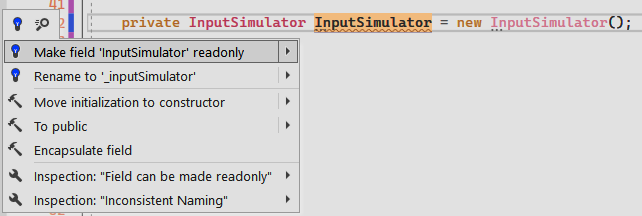
\includegraphics[width=125mm]{images/resharper_refac.png}
	\caption{Refactoring Vorschläge von ReSharper}
	\label{fig:resharper_refactor}
\end{figure}
\FloatBarrier

Alternative Tools für eine derart große Anzahl an unterschiedlichen Sprachen und Funktionen sind aktuell keine auf dem Markt. Kostenlose Alternativen wie \textbf{CodeRush} beschränken sich zumeist auf wenige Sprachen \cite{DocumentationCodeRush}. Allerdings bieten viele IDEs einige dieser Funktionen out of the box an und viele Entwickler arbeiten generell nur mit einer Programmiersprache. Daher können andere, für die jeweilige Programmiersprache geeignete, Tools verwendet werden.